\documentclass[letterpaper]{article} % DO NOT CHANGE THIS
% Anonymous-submission mode; for the camera-ready, drop the [submission]
% option and restore the author block below.
\usepackage[submission]{aaai2026}
\usepackage{times}          % DO NOT CHANGE THIS
\usepackage{helvet}         % DO NOT CHANGE THIS
\usepackage{courier}        % DO NOT CHANGE THIS
\usepackage[hyphens]{url}   % DO NOT CHANGE THIS
\usepackage{graphicx}       % DO NOT CHANGE THIS
% Resolve figures whether the compile root is the repo root (figures/ a sibling
% of paper/) or a flattened Overleaf project (figures/ next to main.tex).
\graphicspath{{figures/}{../figures/}{./}}
\urlstyle{rm}               % DO NOT CHANGE THIS
\def\UrlFont{\rm}           % DO NOT CHANGE THIS
\usepackage{caption}        % DO NOT CHANGE THIS
\frenchspacing              % DO NOT CHANGE THIS
\setlength{\pdfpagewidth}{8.5in}  % DO NOT CHANGE THIS
\setlength{\pdfpageheight}{11in}  % DO NOT CHANGE THIS

% Paper-specific packages (none on the AAAI disallowed list).
\usepackage{amsmath,amssymb}
\usepackage{booktabs}
\usepackage{multirow}
\usepackage{microtype}
\usepackage{natbib}         % AAAI author-year citations; the style file sets
                            % \bibliographystyle{aaai2026} automatically.

\pdfinfo{
/TemplateVersion (2026.1)
}
% Section + subsection numbers (sanctioned by the AAAI template: "May be
% changed to 1 or 2 if section numbers are desired"); the paper cross-references
% subsections, so numbering depth 2 is required for \ref to resolve.
\setcounter{secnumdepth}{2}

% -----------------------------------------------------------------------
\title{One-Step Is Optimal: Unconditional Rectified Flows are\\
       Noise2Noise Denoisers, and Multi-Step Integration Provably Hurts---\\
       A Benchmark and Task-Based Detectability Study on Low-Dose CT}

% Camera-ready author block (hidden by the [submission] option; the style
% file prints ``Anonymous submission'' in its place):
% \author{Tim Sereda}
% \affiliations{\texttt{timgsereda@gmail.com}}
\author{Anonymous submission}
\affiliations{Anonymous submission}
% -----------------------------------------------------------------------

\begin{document}
\maketitle

% -----------------------------------------------------------------------
\begin{abstract}
Iterative and generative denoisers are increasingly deployed on the assumption
that refining a sample over many steps beats a single regression pass.  We prove
the opposite for \emph{label-free} denoising.  An \emph{unconditional} rectified
flow, trained on two noisy observations of the same signal (the Noise2Noise
setting), has a minimiser whose one-step readout is exactly the MMSE
denoiser, recovered with no clean targets, and any multi-step integration
\emph{provably departs} from it---exactly so in a tractable Gaussian model---because
the flow's terminal marginal is the noisy law, not the clean signal.  A
matched-pairing experiment confirms both halves: one-step flow ties a direct
regressor, while multi-step Euler integration monotonically erodes fidelity,
without ever fabricating structure.  Counterintuitively, this failure \emph{grows
with training}: a better-fit velocity integrates more faithfully toward the noisy
terminal law, so multi-step quality degrades as the model improves---a prediction
the departure result makes and the experiments bear out.
The useful ingredient is therefore the decorrelated \emph{pairing}, not the flow
machinery: a one-step regressor on those pairs is our best label-free result
($+1.99$\,dB).  We establish this on \textbf{CTDenoiser}, an open benchmark we use
as a controlled, matched-data testbed for the claim---five architectures across
supervised, similarity- and blind-spot self-supervised, and per-image regimes on
low-dose CT, where the stakes are concrete.  Among label-free methods only the correlated-noise-aware Noise2Sim
beats the noisy baseline, while blind-spot Noise2Void is
flat-to-negative, because CT's spatially correlated noise violates the
pixel-independence these methods assume.  And under a task-based channelized
Hotelling observer, the $\sim$4\,dB PSNR that supervised denoisers do gain
\emph{erodes} low-contrast lesion detectability rather than improving it, a shift
PSNR and SSIM miss.  All code, model definitions, and data-loading utilities will
be released openly (repository link withheld for anonymous review).
\end{abstract}

% -----------------------------------------------------------------------
\section{Introduction}

Iterative and generative denoisers, such as diffusion and flow-matching models, are
increasingly deployed on the assumption that modelling the full distribution of
clean images, and refining a sample over many steps, buys quality over a single
regression pass.  We show that for \emph{label-free} denoising this assumption is
provably counter-productive.  Trained on two independent noisy observations of the
same signal (the Noise2Noise setting), an \emph{unconditional} rectified flow has
a minimiser whose one-step readout is exactly the Noise2Noise MMSE denoiser (a
direct regressor), and we prove that integrating the learned ODE for any positive
time \emph{monotonically increases} denoising error, because the flow's terminal
marginal is the noisy law, not the clean signal.  A matched-data, matched-backbone
experiment confirms both halves: one-step flow ties a direct regressor, and
multi-step Euler integration erodes it monotonically, without ever fabricating
structure.  We establish this on low-dose computed tomography (CT), where the
stakes are concrete: CT's spatially correlated reconstruction noise breaks the
pixel-independence assumption behind blind-spot self-supervision, and a task-based
observer shows the fidelity gains denoisers do achieve can \emph{erode} diagnostic
detectability rather than improve it.

Computed tomography (CT) is a cornerstone of modern medical imaging, but
the ionising radiation dose required for high-quality scans poses a
non-trivial lifetime cancer risk~\cite{brenner2007computed}.  Clinical
practice therefore frequently acquires low-dose CT (LDCT) scans and
applies post-hoc denoising.  The resulting reconstruction quality is
constrained by a fundamental trade-off: aggressive denoising suppresses
quantum noise but blurs fine anatomical structures; insufficient
denoising preserves sharpness but leaves noise that hampers radiological
interpretation.

Deep learning has transformed LDCT denoising.  Convolutional
encoder-decoders~\cite{chen2017lowdose} and
transformers~\cite{wang2022ctformer} now achieve near full-dose image
quality on the TCIA LDCT benchmark~\cite{moen2021low}, while diffusion
and flow-based generative models are beginning to emerge as an
alternative that models the full \emph{distribution} of plausible clean
images rather than a single point estimate.  The harder regime is
\emph{label-free} denoising, where paired full-dose targets are
unavailable; here CT's spatially correlated reconstruction noise breaks the
pixel-independence assumption that underpins blind-spot and downsampling
self-supervision.

Despite this progress, comparing methods fairly is difficult: published
results use heterogeneous preprocessing pipelines, evaluation patches,
normalisation conventions, and metric implementations~\cite{eulig2024benchmark}.
We address this with CTDenoiser, a self-contained benchmark that:

\begin{itemize}
  \item provides a single training loop and evaluation harness usable
        without modification for all five included architectures and five
        supervision regimes (supervised, similarity-based and blind-spot
        self-supervised, and two zero-shot per-image methods);
  \item enforces patient-level train/validation splits to prevent slice
        leakage;
  \item evaluates on full CT slices via overlapped tiling rather than
        held-out patches;
  \item augments the standard pixel-fidelity metrics with GMSD and
        a Residual Spectral Ratio (RSR) to surface the perceptual
        trade-offs of generative denoisers.
\end{itemize}

This benchmark is the substrate for the theoretical result, not an end in
itself: its matched-data, matched-backbone control is precisely what lets the
label-free flow-versus-regression comparison below isolate the \emph{estimator}
from the \emph{pairing}, and turn the one-step-optimality claim into a controlled
test rather than an anecdote.

Our contributions are: (i) a theoretical result---an unconditional rectified
flow trained on Noise2Noise pairs recovers the one-step MMSE denoiser, together
with a finite-step departure proposition proving (exactly, in a tractable
Gaussian model) that multi-step integration monotonically worsens it, with the
counterintuitive corollary that the degradation \emph{grows as the velocity is
better fit} (Section~\ref{sec:method}); (ii) a matched-data,
matched-backbone experiment confirming both halves---one-step flow ties direct
regression while iteration erodes it---on a reproducible five-architecture,
five-regime LDCT benchmark with a corrected full-slice evaluation
(Sections~\ref{sec:inference},~\ref{sec:results}), on which the only label-free
method to reliably beat the noisy input is the correlated-noise-aware Noise2Sim;
and (iii) a task-based, hallucination-aware detectability evaluation---a
channelized Hotelling observer with a corrected noise-power spectrum---showing the
benchmark's PSNR/SSIM gains \emph{erode} low-contrast lesion detectability without
fabricating structure (Section~\ref{sec:detect}).

% -----------------------------------------------------------------------
\section{Related Work}

\paragraph{CNN-based denoisers.}
RED-CNN~\cite{chen2017lowdose} introduced a residual encoder-decoder
with multi-level skip connections and remains a standard baseline.
DnCNN~\cite{zhang2017beyond} demonstrated that a flat stack of
Conv-BN-ReLU layers with a single residual prediction (noise subtraction
rather than clean-image prediction) achieves strong performance on
natural image denoising and transfers well to CT.

\paragraph{Transformer denoisers.}
CTformer~\cite{wang2022ctformer} applies a U-shaped transformer with
Token2Token Dilation (T2TD) blocks that aggregate local neighbourhood
tokens via dilated convolutions interleaved with cyclic spatial shifts.
This allows long-range self-attention without the quadratic memory cost
of global attention on full-resolution feature maps.

\paragraph{Generative approaches.}
Score-based diffusion models~\cite{song2021scorebased} have been applied
to CT denoising~\cite{gao2023corediff} and can produce perceptually
superior results, but inference requires hundreds to thousands of neural
function evaluations (NFEs).  Conditional flow matching~\cite{lipman2022flow,
albergo2022building} reduces this to as few as 10--50 NFEs by learning
straight-line probability paths between source and target distributions,
making it practical for clinical deployment.  Recent few-/single-step
generative denoisers push this further: Poisson Flow Consistency Models
(PFCM)~\cite{hein2025pfcm} distil a generative LDCT denoiser to a single step
and report that an unconstrained generative process introduces substantial
variability across denoised images, motivating fidelity-preserving
sampling---a concern our self-supervised flow addresses by construction
(Section~\ref{sec:method}).  More fundamentally, the perception--distortion
trade-off~\cite{blau2018perception} establishes that minimising distortion
necessarily costs perceptual realism for any distortion measure, the formal
reason a generative denoiser can look realistic while being unfaithful.  A
parallel line makes the link to denoising explicit: an optimally trained
flow-matching velocity yields the one-step MMSE denoiser at each noise
level~\cite{gagneux2025phases,albergo2023stochastic}, and
posterior-mean-then-transport estimators
(PMRF~\cite{ohayon2025pmrf}, InDI~\cite{delbracio2023indi}) separate the MMSE
regression step from the generative transport---conceding that iteration buys
perceptual realism, not distortion.  Section~\ref{sec:method} pushes this to the
label-free regime and finds the transport is not merely optional but a liability
for the denoising objective.

\paragraph{Self-supervised and zero-shot denoisers.}
When paired full-dose targets are unavailable, denoisers can be trained
from noisy data alone.  Noise2Noise~\cite{lehtinen2018noise2noise} showed
that mapping between two independent noisy observations of the same scene
recovers the clean signal in expectation.  Noise2Void~\cite{krull2019noise2void}
removes the need for a second observation via a blind-spot scheme that
withholds each target pixel from the network's receptive field, but it
assumes pixel-wise \emph{independent} noise---an assumption violated by CT,
whose reconstruction noise is spatially correlated.
Neighbor2Neighbor~\cite{huang2021neighbor2neighbor} manufactures a
Noise2Noise pair from a single image by sub-sampling neighbouring pixels,
inheriting the same independence assumption.  Two lines of work address
correlated noise directly: Noise2Sim~\cite{niu2020noise2sim} learns to map
between the centre pixels of self-similar non-local patches, suppressing
correlated as well as independent noise and remaining asymptotically
equivalent to supervised learning; and Zero-Shot Noise2Noise
(ZS-N2N)~\cite{mansour2023zsn2n} trains a tiny network per image from a
downsampled Noise2Noise pair, requiring no external data, no noise model,
and no pretraining.  In the vision literature, asymmetric pixel-shuffle
downsampling (AP-BSN)~\cite{lee2022apbsn} breaks spatial correlation with a
large training stride while preserving detail with a small inference stride,
the mechanism most correlated-noise blind-spot successors build on.  More
recently, Filter2Noise~\cite{sun2025filter2noise} couples self-supervised
single-image training with an interpretable attention-guided bilateral
filter designed specifically for LDCT, and WIA-LD2ND~\cite{zhao2024wia}
performs self-supervised LDCT denoising in the wavelet domain.  A unifying view
is Noise2Score~\cite{kim2021noise2score}: self-supervised denoising reduces to
score estimation, and Tweedie's formula then returns the posterior mean
$\mathbb{E}[s\mid x]$, placing Noise2Noise, Noise2Void, and SURE under one
estimator---the same MMSE target our flow reaches in a single step
(Section~\ref{sec:method}), but via score/Tweedie rather than the flow velocity.
Our benchmark includes Noise2Void, ZS-N2N, and Filter2Noise as label-free
baselines and adds Noise2Sim as the correlated-noise-aware extension.

\paragraph{Task-based and hallucination-aware evaluation.}
\label{sec:rw-taskbased}
Pixel-fidelity metrics such as PSNR and SSIM are increasingly recognised as
poor proxies for diagnostic quality on medical images, both because they
misrank novel restoration algorithms~\cite{breger2025reassess} and because
they do not track radiologist perception of denoised
CT~\cite{lee2025ldctiqa}.  The more rigorous standard is \emph{task-based}
assessment: model observers such as the Channelized Hotelling Observer (CHO)
estimate detectability ($d'$, AUC) on signal-known-exactly /
background-known-statistically tasks.  Bhadra et al.~\cite{bhadra2021halluc}
gave the first formal definition of hallucination in tomographic
reconstruction via the measurement / null-space decomposition, and Tivnan et
al.~\cite{tivnan2024halluc} introduced a Hallucination Index for generative
reconstruction that distinguishes added noise from added structure.  Applied
to denoisers specifically, Li et al.~\cite{li2021detection} showed that deep
denoising can \emph{destroy} task-relevant information even as conventional
image-quality metrics improve, and Kc \& Zeng~\cite{kc2024lgcho} found that
quarter-dose denoised CT can beat full-dose on PSNR and SSIM while remaining
\emph{inferior} on low-contrast detectability.  These works motivate the
hallucination-aware, detectability-based evaluation we report on this
benchmark's supervised and self-supervised models in
Section~\ref{sec:detect}.

\paragraph{Evaluation metrics.}
PSNR and SSIM are ubiquitous but favour pixel-level fidelity, potentially
penalising generative models that hallucinate plausible-but-incorrect
high-frequency detail.  Perceptual metrics such as
LPIPS~\cite{zhang2018unreasonable} and the noise power spectrum
(NPS)~\cite{solomon2012characterization} are more appropriate for
evaluating perceptual quality and texture authenticity, respectively.

% -----------------------------------------------------------------------
\section{Methods}

\subsection{Data and Preprocessing}

We use the TCIA LDCT-and-Projection-Data
dataset~\cite{moen2021low}, which contains paired low-dose and full-dose
reconstructions.  DICOM slices are read with \texttt{pydicom}, sorted by
$z$-position, and converted to Hounsfield units (HU).  HU values are
windowed to $[0, 1]$ via

\begin{equation}
  x = \operatorname{clamp}\!\left(\frac{u + b}{s},\; 0,\; 1\right),
  \label{eq:hu-norm}
\end{equation}

where $u$ is the raw HU value and $(b,s)$ is a fixed anatomy window preset.
The processed arrays are cached as an HDF5 file (one dataset per
patient/dose level) for efficient random access during training.

Patients are split at the patient level (not the slice level) into
training and validation sets using a configurable fraction
($\text{val\_fraction}=0.2$ by default) and a fixed random seed, preventing
any slice from a validation patient appearing in training.  During
training, $64\times64$ patches are sampled uniformly at random from each
slice.  During validation, full CT slices of variable size are processed
via the overlapped-tiling inference strategy described in
Section~\ref{sec:inference}.

\subsection{Architectures}

\paragraph{RED-CNN.}
Chen et al.'s~\cite{chen2017lowdose} Residual Encoder-Decoder CNN uses
$5\times5$ convolutions throughout.  The encoder consists of five
convolutional layers (96 filters each), and the decoder mirrors this
with five transposed-convolutional layers.  Skip connections are added at
three depths, and all activations use ReLU.

\paragraph{DnCNN.}
Zhang et al.'s~\cite{zhang2017beyond} denoising CNN uses 17 layers of
$3\times3$ convolutions.  The first layer has no batch normalisation;
intermediate layers each apply Conv-BN-ReLU; the final layer has neither.
The network predicts the noise component $n$ and returns
$\hat{x} = x - n$, a residual-learning formulation.

\paragraph{CTformer.}
Wang et al.'s~\cite{wang2022ctformer} architecture tokenises the input
with a strided convolution, applies a symmetric
encoder-bottleneck-decoder of Transformer blocks interleaved with
Token2Token Dilation (T2TD) modules, then detokenises with a transposed
convolution.  Each T2TD block applies a cyclic spatial shift and a dilated
re-tokenisation before multi-head self-attention.

\paragraph{U-Net.}
Our U-Net baseline uses three encoder stages, a two-layer bottleneck, and a
symmetric decoder with bilinear upsampling and concatenated skip
connections.  It is included for ablation: it shares the overall shape of
the velocity network inside our CFM model, so comparing U-Net (MSE) versus
CFM (flow-matching) isolates the contribution of the generative training
objective.

\paragraph{Conditional Flow Matching (CFM).}
\label{sec:cfm}
Conditional flow matching~\cite{lipman2022flow} frames denoising as
learning a time-dependent vector field $v_\theta$ that transports a
source distribution $p_0$ (LDCT images) to a target distribution $p_1$
(full-dose images).  The \emph{rectified flow}
formulation~\cite{liu2022flow} uses straight-line paths, so the
conditional vector field is simply

\begin{equation}
  v^* = x_1 - x_0,
  \label{eq:rectified-target}
\end{equation}

constant along the path.  The training objective is

\begin{equation}
  \mathcal{L}_\text{CFM}(\theta)
  = \mathbb{E}_{t, x_0, x_1}\bigl[\|v_\theta(x_t,\, x_0,\, t) - (x_1 - x_0)\|^2\bigr],
  \label{eq:cfm-loss}
\end{equation}

where $t \sim \mathcal{U}[0,1]$, the interpolant is
$x_t = (1-t)x_0 + t\,x_1$, and $x_0$ (the noisy LDCT patch) is passed as a
conditioning channel: the velocity network input is the two-channel
concatenation $[x_t; x_0]$.  At inference we integrate the learned ODE with
$K$ forward-Euler steps initialised at the noisy input.  This conditional
formulation requires paired clean targets and is the supervised baseline we
contrast against in Section~\ref{sec:method}.

\subsection{Training}

All models use the Adam optimiser at learning rate $10^{-4}$ and batch
size 4 (patches of $64\times64$).  Deterministic models (RED-CNN, DnCNN,
CTformer, U-Net) minimise pixel-level MSE; CFM uses
$\mathcal{L}_\text{CFM}$ (Eq.~\eqref{eq:cfm-loss}).

\paragraph{Supervision regimes.}
\emph{Supervised} training uses paired full-dose targets.
\emph{Noise2Void}~\cite{krull2019noise2void} replaces a fraction
$\rho=0.02$ of pixels per patch with a random neighbour within radius
$r=2$ and computes the loss against the original noisy value at those
blind-spot locations only.  \emph{Noise2Sim}~\cite{niu2020noise2sim}
constructs a self-supervised target from the centre pixels of non-local
self-similar patches.  \emph{ZS-N2N}~\cite{mansour2023zsn2n} is
architecture-agnostic: for each image a fresh three-layer residual network
($21.3\mathrm{K}$ parameters) is optimised for 2000 iterations on a
diagonally-downsampled Noise2Noise pair, then discarded.
\emph{Filter2Noise}~\cite{sun2025filter2noise} similarly optimises a small
single-image filter at test time.  Because CFM requires paired clean
targets, its blind-spot and similarity variants are undefined and omitted.

\subsection{Inference}
\label{sec:inference}

Full CT slices vary in size and are typically larger than the training
patch size.  We use an overlapped-tiling strategy to eliminate
grid-boundary artefacts: each patch of size $P\times P$ overlaps its
neighbours by a margin $m = P/4$, and predictions in the overlap region are
blended by a weighted mean over patch contributions.  Patches at the image
boundary retain their full extent: the margin is discarded only on sides
shared with a neighbouring patch, never on a side that abuts the image
edge.  An earlier version that discarded the margin on \emph{all} sides
left each slice's outer $m$-pixel border unpopulated (set to zero); because
the identity baseline does not pass through this routine, that artefact
biased the reconstruction metrics of every trained model.  All results
below use the corrected tiling.

\subsection{Evaluation Metrics}

\paragraph{PSNR / SSIM / RMSE.}
PSNR uses data range $R=1$ after normalisation; SSIM~\cite{wang2004image}
uses a Gaussian window ($\sigma=1.5$, window $11$); RMSE is
$\sqrt{\text{MSE}}$.

\paragraph{Gradient Magnitude Similarity Deviation (GMSD).}
GMSD~\cite{xue2014gradient} computes gradient magnitudes of the predicted
and reference images with Prewitt kernels and reports the standard
deviation of the gradient-magnitude-similarity map; lower is better and no
pretrained features are required.

\paragraph{Residual Spectral Ratio (RSR).}
\begin{equation}
  \text{RSR} = \frac{\mathbb{E}\bigl[|\mathcal{F}(\hat{x}-x_1)|^2\bigr]}
                    {\mathbb{E}\bigl[|\mathcal{F}(x_1)|^2\bigr] + \varepsilon},
  \label{eq:nps}
\end{equation}
where $\mathcal{F}$ is the 2-D DFT.  This measures the fraction of
clean-image spectral energy present in the residual error and is sensitive
to hallucinated high-frequency texture~\cite{gao2023corediff} that PSNR and
SSIM may miss.  RSR is a frequency-domain \emph{error} ratio against the
reference and should not be confused with the conventional CT noise-power
spectrum (NPS), which characterises the spectrum of the noise itself,
estimated from uniform-region ROIs; the latter is what we report as the NPS
radial centroid in the task-based evaluation of Section~\ref{sec:detect}.

% -----------------------------------------------------------------------
\section{Experiments}

\subsection{Setup}

Experiments use the TCIA LDCT-and-Projection-Data dataset~\cite{moen2021low}
(abdomen window) with patient-level splits ($\sim$$6{,}500$ training and
$\sim$$1{,}600$ validation slices per split).  The main benchmark
(Table~\ref{tab:results}) reports the mean over three such splits; the SSFlow
ablations (Section~\ref{sec:method}) use a single split (seed 0).  Trained models
run for 50 epochs with patch size 64, batch size 4, and Adam at $10^{-4}$; the
CFM model integrates the ODE with $K=20$ Euler steps during training and 5 at
evaluation.  The per-image methods (ZS-N2N, Filter2Noise) optimise one
network per validation image and are model-agnostic.  Validation metrics
are computed over full slices using the corrected overlapped inference of
Section~\ref{sec:inference} with margin $P/4 = 16$.  We report the gain
($\Delta$) of each metric relative to the unprocessed \emph{LDCT input},
the floor every method must beat.

\subsection{Results}
\label{sec:results}

\begin{table*}[t]
  \centering
  \small
  \caption{\textbf{Main benchmark} (\texttt{sweep.yml}): validation results on
           TCIA LDCT (abdomen; patient-level $3$-seed splits, $50$ epochs),
           grouped by supervision regime.  Mean\,$\pm$\,s.d.\ over $3$ seeds on
           full slices via overlapped tiling (corrected border handling).  The
           PSNR column gives the absolute value with the gain over each split's
           \emph{LDCT input} floor in parentheses (mean floor $30.25$\,dB).  All
           five architectures are complete over $3$ seeds.  CFM requires paired
           targets, so it has no blind-spot or similarity variant.  Per-image
           methods (ZS-N2N, Filter2Noise) are in Table~\ref{tab:sweep-periimage};
           the label-free SSFlow and its one- vs.\ multi-step ablation are in
           Section~\ref{sec:method}.  \textbf{Bold}: best $\Delta$PSNR per
           supervision block.  $\uparrow$/$\downarrow$: higher/lower is better.}
  \label{tab:results}
  \begin{tabular}{llrccccc}
    \toprule
    \textbf{Model} & \textbf{Supervision} & \textbf{Params} &
    PSNR\,$\uparrow$ (\,$\Delta$) & SSIM\,$\uparrow$ & RMSE\,$\downarrow$ &
    GMSD\,$\downarrow$ & RSR\,$\downarrow$ \\
    \midrule
    LDCT input & --- (no denoising) & --- & $30.25$ & $0.876$ & $0.0320$ & $0.174$ & $0.0115$ \\
    \midrule
    RED-CNN~\cite{chen2017lowdose}   & Supervised & $1.85\mathrm{M}$ & \textbf{34.50 \,($+4.25{\pm}0.23$)} & $0.927{\pm}0.013$ & $0.0194$ & $0.167$ & $0.0041$ \\
    U-Net                            & Supervised & $1.95\mathrm{M}$ & 34.26 \,($+4.02{\pm}0.22$) & $0.925{\pm}0.014$ & $0.0199$ & $0.188$ & $0.0044$ \\
    DnCNN~\cite{zhang2017beyond}     & Supervised & $0.56\mathrm{M}$ & 34.23 \,($+3.99{\pm}0.18$) & $0.924{\pm}0.014$ & $0.0200$ & $0.198$ & $0.0044$ \\
    CFM~\cite{lipman2022flow}        & Supervised & $2.11\mathrm{M}$ & 33.09 \,($+2.84{\pm}0.22$) & $0.915{\pm}0.013$ & $0.0228$ & $0.192$ & $0.0057$ \\
    CTformer~\cite{wang2022ctformer} & Supervised & $0.40\mathrm{M}$ & 32.01 \,($+1.77{\pm}0.35$) & $0.904{\pm}0.013$ & $0.0255$ & $0.249$ & $0.0070$ \\
    \midrule
    U-Net                            & Noise2Sim~\cite{niu2020noise2sim} & $1.95\mathrm{M}$ & \textbf{32.08 \,($+1.83{\pm}0.08$)} & $0.901{\pm}0.015$ & $0.0259$ & $0.174$ & $0.0075$ \\
    RED-CNN~\cite{chen2017lowdose}   & Noise2Sim~\cite{niu2020noise2sim} & $1.85\mathrm{M}$ & 32.05 \,($+1.81{\pm}0.10$) & $0.901{\pm}0.015$ & $0.0259$ & $0.163$ & $0.0075$ \\
    DnCNN~\cite{zhang2017beyond}     & Noise2Sim~\cite{niu2020noise2sim} & $0.56\mathrm{M}$ & 31.93 \,($+1.69{\pm}0.09$) & $0.898{\pm}0.015$ & $0.0263$ & $0.187$ & $0.0078$ \\
    CTformer~\cite{wang2022ctformer} & Noise2Sim~\cite{niu2020noise2sim} & $0.40\mathrm{M}$ & 31.04 \,($+0.79{\pm}0.13$) & $0.887{\pm}0.018$ & $0.0289$ & $0.232$ & $0.0092$ \\
    \midrule
    RED-CNN~\cite{chen2017lowdose}   & Noise2Void~\cite{krull2019noise2void} & $1.85\mathrm{M}$ & \textbf{30.67 \,($+0.42{\pm}0.06$)} & $0.883{\pm}0.018$ & $0.0303$ & $0.177$ & $0.0103$ \\
    U-Net                            & Noise2Void~\cite{krull2019noise2void} & $1.95\mathrm{M}$ & 30.54 \,($+0.29{\pm}0.04$) & $0.883{\pm}0.018$ & $0.0307$ & $0.198$ & $0.0104$ \\
    DnCNN~\cite{zhang2017beyond}     & Noise2Void~\cite{krull2019noise2void} & $0.56\mathrm{M}$ & 30.19 \,($-0.06{\pm}0.03$) & $0.875{\pm}0.018$ & $0.0321$ & $0.224$ & $0.0116$ \\
    CTformer~\cite{wang2022ctformer} & Noise2Void~\cite{krull2019noise2void} & $0.40\mathrm{M}$ & 29.89 \,($-0.36{\pm}0.23$) & $0.862{\pm}0.015$ & $0.0328$ & $0.269$ & $0.0118$ \\
    \bottomrule
  \end{tabular}
\end{table*}

Table~\ref{tab:results} yields three findings.  \textbf{First}, supervised
denoising gains $\sim$4\,dB PSNR over the noisy input, and RED-CNN, U-Net, and
DnCNN finish within $0.3$\,dB of one another despite a $3\times$ range in
parameter count; the transformer (CTformer, $+1.77$\,dB) and the generative flow
(CFM, $+2.84$\,dB) both trail the CNNs even with paired targets, so the objective
and a simple convolutional inductive bias dominate the backbone.
\textbf{Second}, among label-free methods only the correlated-noise-aware
Noise2Sim consistently exceeds the noisy floor ($+1.7$ to $+1.8$\,dB), whereas
blind-spot Noise2Void is flat-to-negative ($-0.06$\,dB on DnCNN); this is direct
evidence that FBP-correlated CT noise violates the pixel-independence assumption
these methods rely on.  \textbf{Third}, a $\sim$2\,dB gap remains between the best
label-free method and the supervised upper bound, quantifying the headroom
for correlated-noise-aware self-supervision---the gap our self-supervised
rectified flow (SSFlow) targets in Section~\ref{sec:method}.

\begin{figure*}[t]
  \centering
  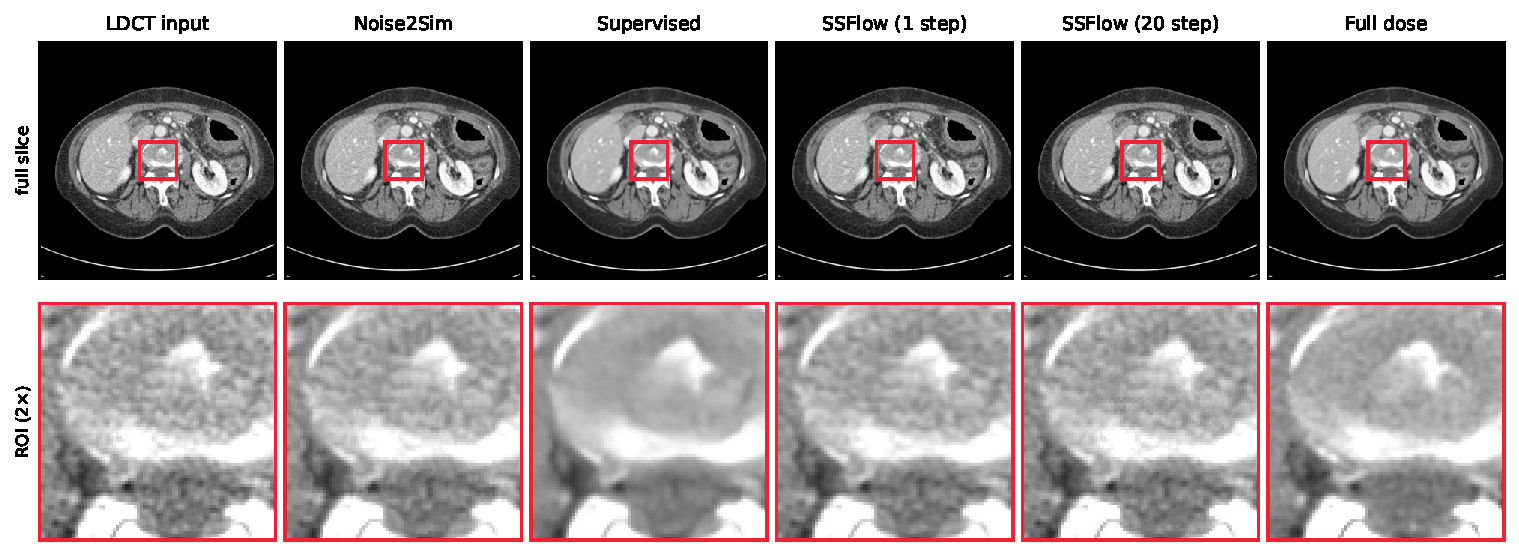
\includegraphics[width=\textwidth]{qualitative.pdf}
  \caption{\textbf{Qualitative comparison} on a held-out abdomen slice (top: full
           slice with the ROI boxed; bottom: $2\times$ ROI).  The supervised model
           removes the most noise but imparts the blotchy, low-frequency
           ``waxy'' texture that the NPS-centroid shift quantifies
           (Section~\ref{sec:detect}); Noise2Sim preserves finer texture; and
           multi-step SSFlow visibly drifts back toward the noisy input relative to
           its one-step readout, as the departure result predicts.}
  \label{fig:qual}
\end{figure*}

\paragraph{Per-fold stability.}
The regime ordering holds fold-by-fold and is established early in training: a
reduced 15-epoch replication on the same three folds
(Appendix~\ref{app:supp-tables}, Table~\ref{tab:cv}) reproduces it---supervised
$+4.0$ to $+4.2$\,dB, Noise2Sim the only label-free method clearing the floor
($+1.74{\pm}0.09$\,dB on RED-CNN), and the rest within noise
($|\Delta\text{PSNR}|\le0.32$\,dB)---with absolute PSNR already within
$\sim$0.1\,dB of the 50-epoch benchmark (RED-CNN supervised $34.43$ vs.\
$34.50$\,dB).

\subsection{Task-based detectability}
\label{sec:detect}

\begin{figure*}[t]
  \centering
  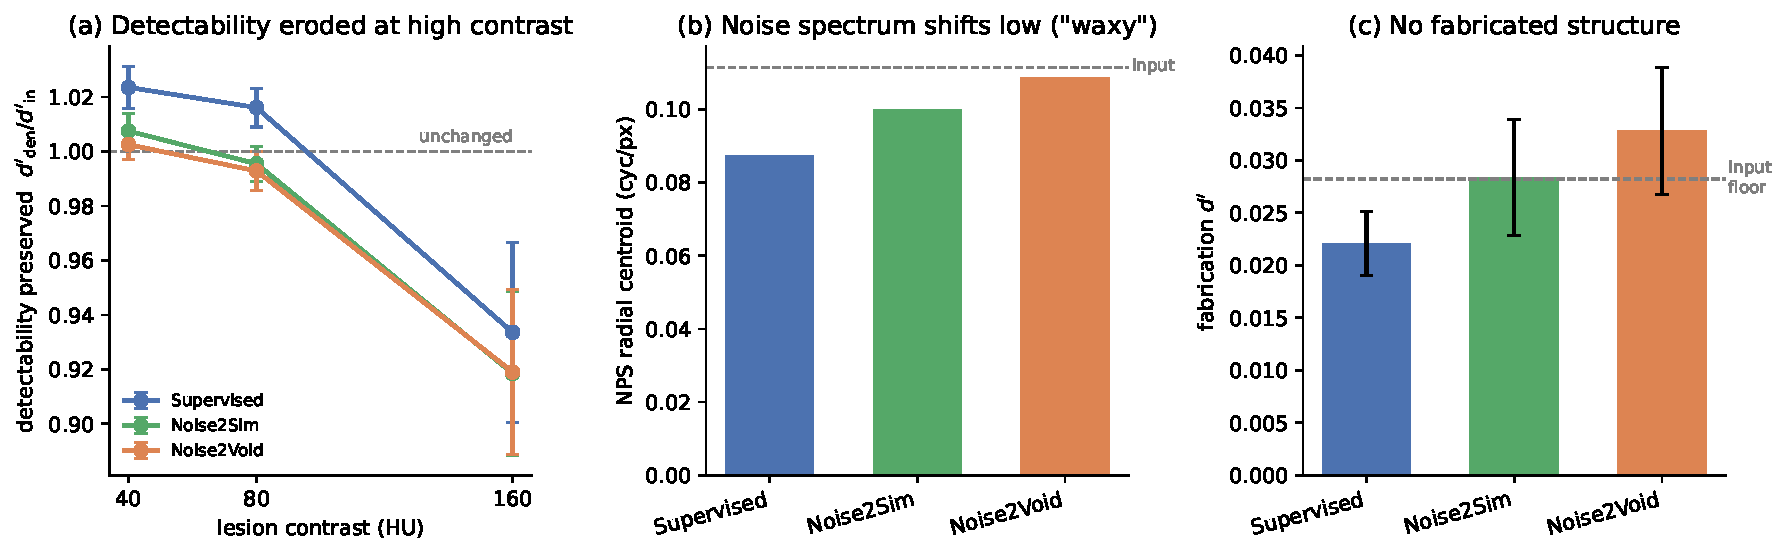
\includegraphics[width=\textwidth]{detectability.pdf}
  \caption{\textbf{Task-based detectability} on the benchmark CNNs (mean over $3$
           architectures $\times$ $3$ seeds).  \emph{(a)} CHO detectability
           preserved $d'_\text{den}/d'_\text{in}$ vs lesion contrast: the erosion
           concentrates at the high-contrast operating point---precisely where
           PSNR/SSIM report their largest, most confident gains.  \emph{(b)} The
           denoised NPS radial centroid falls below the input (dashed)---the
           low-frequency ``waxy'' texture---most for the supervised models.
           \emph{(c)} Fabrication $d'$ stays at the signal-absent input floor
           (dashed) for every regime: detectability is eroded \emph{without}
           inventing structure.}
  \label{fig:detect}
\end{figure*}

Pixel-fidelity gains need not be diagnostic gains.  We test this directly with
a Channelized Hotelling Observer (CHO) on a signal-known-exactly /
background-known-statistically (SKE/BKS) task.  No CT forward projector is
needed: because the dataset provides real paired low/full acquisitions, the
real spatially-correlated FBP noise is $n = x_\text{low} - x_\text{full}$, so a
signal-present low-dose image is \emph{literally} $x_\text{low} + s$ for a known
lesion $s$ (the same correlated noise is re-attached by construction), and the
signal-absent image is the untouched acquisition.  We insert Gaussian lesions of
radius $4$\,px at $40/80/160$\,HU on flat in-body sites ($6$ per slice, $200$
slices per run), extract present/absent ROIs at the \emph{input}, \emph{denoised}
and \emph{clean} stages, channelise with ten Laguerre-Gauss channels, and compute
the detectability index $d'$.  The observer is validated against the closed-form
white-noise value $d' = \lVert s\rVert / \sigma$ as a unit test before use.  We
run it on the completed three-seed benchmark models of
Table~\ref{tab:results} (the three CNN architectures) and report the
mean over architectures and seeds; CTformer reproduces the same erosion and is
held out only to keep the aggregate architecturally homogeneous.  The
per-image methods (ZS-N2N, Filter2Noise) are omitted---each CHO realisation would
retrain their per-image network thousands of times---and the generative
SSFlow/CFM detectability, which can \emph{fabricate} as well as erode, is reported
separately.

\begin{table*}[t]
  \centering
  \small
  \caption{Task-based detectability on the completed benchmark models
           (Table~\ref{tab:results}); mean over $3$ CNN architectures
           $\times$ $3$ seeds ($27$ runs; CTformer, now complete, reproduces the
           same erosion and is held out to keep the aggregate CNN-only).
           \emph{Top:} CHO detectability index $d'$ for the noisy
           input (floor) and clean reference (ceiling) at three lesion
           contrasts; these are method-independent and carry a large
           between-split (patient-cohort) s.d.\ ($\pm1.3$ at $160$\,HU), which is
           why we report the ratio below.  \emph{Bottom:} detectability
           \emph{preserved}, $d'_\text{denoised}/d'_\text{input}$
           (mean\,$\pm$\,s.d.; $1.0=$ unchanged, $<1=$ eroded); the denoised
           noise-power-spectrum radial centroid (input $0.112$; lower $=$ more
           low-frequency ``waxy'' texture); and the \emph{fabrication} $d'$ from
           a CHO run on \emph{signal-absent} ROIs (input floor $0.028$; $>$floor
           $=$ invented structure).  Architecture differences are within s.d.,
           so rows are aggregated by supervision regime.  $d'_\text{denoised}$ is
           below $d'_\text{input}$ in all $27$ runs and never exceeds the clean
           ceiling, while fabrication $d'$ never rises above the floor.}
  \label{tab:detect}
  \begin{tabular}{lccccc}
    \toprule
     & \multicolumn{3}{c}{lesion contrast (HU)} & NPS & fab. \\
    \cmidrule(lr){2-4}
     & $40$ & $80$ & $160$ & centroid\,$\downarrow$ & $d'\,\downarrow$ \\
    \midrule
    \multicolumn{6}{l}{\emph{Reference $d'$ (method-independent)}} \\
    \quad input (floor)   & $1.51$ & $3.03$ & $6.06$ & $0.112$ & $0.028$ \\
    \quad clean (ceiling) & $1.54$ & $3.09$ & $6.18$ & --- & --- \\
    \midrule
    \multicolumn{6}{l}{\emph{Detectability preserved $d'_\text{den}/d'_\text{in}$}} \\
    \quad Supervised & $1.024\,{\pm}\,0.008$ & $1.016\,{\pm}\,0.007$ & $0.934\,{\pm}\,0.033$ & $0.087\,{\pm}\,0.004$ & $0.022\,{\pm}\,0.003$ \\
    \quad Noise2Sim  & $1.008\,{\pm}\,0.006$ & $0.995\,{\pm}\,0.006$ & $0.919\,{\pm}\,0.030$ & $0.100\,{\pm}\,0.005$ & $0.028\,{\pm}\,0.006$ \\
    \quad Noise2Void & $1.003\,{\pm}\,0.006$ & $0.993\,{\pm}\,0.007$ & $0.919\,{\pm}\,0.030$ & $0.109\,{\pm}\,0.006$ & $0.033\,{\pm}\,0.006$ \\
    \bottomrule
  \end{tabular}
\end{table*}

Table~\ref{tab:detect} and Figure~\ref{fig:detect} show four things.
\textbf{First}, the detectability
\emph{headroom} is small: the clean reference exceeds the noisy input by only
$\sim$2\% ($d' = 6.18$ vs.\ $6.06$ at $160$\,HU), so at this dose the inserted
lesions are nearly as detectable in the noisy image as in the noise-free one.
This narrow headroom is not an artefact of the test but the clinically relevant
regime: at a realistic LDCT dose the noise floor already leaves supra-threshold
lesions detectable, so the question is not whether denoising \emph{recovers} lost
detectability but whether it \emph{preserves} it---and, as the next finding shows,
even where headroom does exist (high contrast) the denoisers spend it, eroding
detectability rather than closing the gap to the clean ceiling.
\textbf{Second}, although these same models gain $4.0$--$4.3$\,dB PSNR
(supervised) and $1.7$--$1.8$\,dB (Noise2Sim) over the input
(Table~\ref{tab:results}), none improves detectability at the
supra-threshold operating point: $d'_\text{denoised} < d'_\text{input}$ in all
$27$ runs---a $7$--$8\%$ loss at $160$\,HU---and none exceeds the clean ceiling,
while the fabrication $d'$ on signal-absent ROIs stays at its floor
($0.022$--$0.033$ vs.\ the $0.028$ input floor), so the deterministic denoisers
\emph{erode} detectability without \emph{fabricating} it.  The erosion is
contrast-dependent: near the detection threshold ($40$\,HU) detectability is
preserved to within $1$--$2\%$, so the loss concentrates precisely at the
high-contrast operating point where PSNR and SSIM report their largest, most
confident gains.  \textbf{Third}, the supervised models that win most on PSNR
also shift the noise-power-spectrum centroid furthest toward low frequency
($0.112 \!\to\! 0.087$, a $22\%$ drop, vs.\ $0.112 \!\to\! 0.109$ for
Noise2Void), the blotchy / ``waxy'' texture radiologists distrust and that is
visible in the qualitative panel (Figure~\ref{fig:qual}).
\textbf{Fourth}, the differences \emph{between} supervision regimes are not
statistically resolved at this sample size: the preserved-detectability ratios
at $160$\,HU ($0.934\,{\pm}\,0.033$ supervised, $0.919\,{\pm}\,0.030$
Noise2Sim, $0.919\,{\pm}\,0.030$ Noise2Void) overlap well within one standard
deviation, so the data support the \emph{erosion} claim---every regime sits
below $1.0$---but not a fine-grained regime-vs-regime detectability ranking;
only the NPS-centroid shift cleanly separates supervised from blind-spot
training.  Reporting the \emph{preserved} ratio
$d'_\text{denoised}/d'_\text{input}$ rather than the raw index matters here: it
cancels the large between-split variation in absolute $d'$ (s.d.\ $\pm1.31$ at
$160$\,HU) and is stable across seeds ($\pm0.003$--$0.033$), isolating the
denoiser's effect.  None of this contrast-dependent erosion or texture shift
appears in PSNR or SSIM, which rise monotonically; task-based $d'$ is therefore
a necessary complement to them, not an optional one.

% -----------------------------------------------------------------------
\section{An Unconditional Rectified Flow is a One-Step Noise2Noise Denoiser}
\label{sec:method}

The results above leave a $\sim$2\,dB gap between the best label-free
method and supervised training.  Our methodological contribution is a pair of
results: the velocity field of an \emph{unconditional} rectified flow, trained on
two noisy observations of the same signal, has a minimiser that recovers the
Noise2Noise posterior mean in a \emph{single} step (Section~\ref{sec:rf-n2n})---no
clean targets, no ODE integration---and any multi-step integration \emph{provably
departs} from that optimum.  We instantiate the one-step result as SSFlow, a
denoiser for the correlated noise of FBP-reconstructed LDCT
(Section~\ref{sec:ss-pairs}): it pairs the unconditional flow with a
\emph{similarity-based} construction of the noisy pairs that keeps the paired
noise independent despite spatial correlation.  A matched-pairing ablation
(Section~\ref{sec:ss-pairs}) confirms both results---one-step flow ties a direct
regressor while multi-step refinement monotonically hurts---so SSFlow is best
read as the empirical realisation of the one-step result, and the decorrelated
pairing, not the flow, is what carries it.

\subsection{Rectified flow as a Noise2Noise estimator}
\label{sec:rf-n2n}
Let $s$ be the (unobserved) clean slice and let $x_0=s+n_0,\ x_1=s+n_1$ be
two noisy observations with $\mathbb{E}[n_i\mid s]=0$ and
$n_0\perp n_1\mid s$.  Using the same straight-line interpolant
$z_t=(1-t)x_0+t\,x_1$ as Eq.~\eqref{eq:rectified-target}, we train an
\emph{unconditional} velocity network $v_\theta(z,t)$ (inputs: the
interpolant $z$ and time $t$ only, in contrast to the conditional field of
Eq.~\eqref{eq:cfm-loss}) with

\begin{equation}
  \mathcal{L}(\theta)=
  \mathbb{E}_{s,n_0,n_1,\,t\sim\mathcal{U}[0,1]}
  \big\|\,v_\theta(z_t,t)-(x_1-x_0)\,\big\|^2 .
  \label{eq:ss-loss}
\end{equation}

\paragraph{Proposition.}
The minimiser of \eqref{eq:ss-loss} is the conditional expectation
$v^\star(z,t)=\mathbb{E}[\,x_1-x_0\mid z_t=z\,]$.  At $t=0$, $z_0=x_0$, so

\begin{equation}
  x_0 + v^\star(x_0,0)
  = \mathbb{E}[x_1\mid x_0]
  = \mathbb{E}[s\mid x_0],
  \label{eq:ss-mmse}
\end{equation}

the MMSE denoiser.  The last equality is the key step: by the tower property,
$\mathbb{E}[x_1\mid x_0]=\mathbb{E}\!\left[\mathbb{E}[x_1\mid s,x_0]\mid
x_0\right]=\mathbb{E}\!\left[s+\mathbb{E}[n_1\mid s,x_0]\mid x_0\right]
=\mathbb{E}[s\mid x_0]$, where $\mathbb{E}[n_1\mid s,x_0]=\mathbb{E}[n_1\mid
s]=0$ because $n_1\perp n_0\mid s$ (so conditioning on $x_0=s+n_0$ adds
nothing beyond $s$) and $\mathbb{E}[n_i\mid s]=0$.  A single velocity
evaluation thus recovers the Noise2Noise~\cite{lehtinen2018noise2noise}
optimum from noisy pairs alone.

This composes two established facts in a setting where neither has been stated
together: the flow-matching denoising identity---an optimally trained velocity
yields the one-step MMSE estimator $\mathbb{E}[x_1\mid x_t]$ at each
level~\cite{gagneux2025phases,albergo2023stochastic}---and the Noise2Noise
conditional-mean identity~\cite{lehtinen2018noise2noise}.  Prior statements of
the former assume a \emph{clean} target $x_1$; the label-free, symmetric
two-noisy-realisation case ($\mathbb{E}[x_1\mid s]=\mathbb{E}[x_0\mid s]=s$) is
the delta, and it is what makes the one-step map a \emph{self-supervised} MMSE
denoiser.  The equivalence is specific to the $L_2$/velocity-MSE objective
(whose minimiser is the conditional mean, not the median or mode) and to the
\emph{restoration} objective---the opposite of the Ambient Diffusion
regime~\cite{daras2023ambient}, where noisy-only training deliberately
\emph{samples} the clean distribution rather than collapsing to its mean.  It is
a population-level identity at the optimum; how far a finite-capacity,
finite-step flow \emph{departs} from it is the empirical question
Section~\ref{sec:ss-pairs} answers---and it departs by losing to direct
regression.

\paragraph{Why the flow must be unconditional.}
If the network is additionally given $x_0$ (as in
Eq.~\eqref{eq:cfm-loss}), then $(z_t,x_0,t)$ determines the target exactly,
$x_1=(z_t-(1-t)x_0)/t$: the regression target is fully observed and the
network reproduces the \emph{noisy} $x_1$ rather than averaging over it,
destroying \eqref{eq:ss-mmse}.  Dropping the conditioning makes each $z_t$
consistent with many pairs, forcing the network to predict their average
velocity, where the independent noise cancels.

\subsection{Similarity-based pairs and inference}
\label{sec:ss-pairs}
Equation~\eqref{eq:ss-mmse} requires two observations whose noise is
independent given the signal.  FBP smears each detector reading across
neighbouring pixels, so spatial-neighbour pairs
(Neighbor2Neighbor~\cite{huang2021neighbor2neighbor},
ZS-N2N~\cite{mansour2023zsn2n}) are only valid when the noise correlation
length is below the pixel pitch.  We instead adopt the non-local
construction of Noise2Sim~\cite{niu2020noise2sim}: for each query patch we
retrieve its $K$ most similar patches elsewhere in the slice, \emph{excluding}
a radius $r$ around the query so matched patches lie beyond the noise
correlation length.  Self-similarity matches the signal while spatial
separation decorrelates the noise, yielding a valid pair $(x_0,x_1)$ from a
single image; $r$ is the key correlated-noise hyper-parameter.  At
inference, the one-step estimate is $\hat s = x + v_\theta(x,0)$, optionally
refined with a few Euler steps of the learned ODE initialised at the noisy
input; we do \emph{not} integrate to the noisy endpoint distribution.

\paragraph{Multi-step refinement provably departs from the optimum.}
The one-step readout is exact \emph{only} at $t{=}0$; integrating further
provably increases denoising error, because the flow's terminal marginal is the
\emph{noisy} law $p_1$, not the clean signal.  We make this precise in the
tractable jointly-Gaussian model (per spectral mode: signal variance
$\sigma_s^2$, independent noise variance $\sigma_n^2$ on each observation), where
$v^\star$ is linear and the ODE $\dot z=v^\star(z,t)$ integrates in closed form to
$\hat z(t)=x_0\sqrt{(\sigma_s^2+\gamma(t)\sigma_n^2)/(\sigma_s^2+\sigma_n^2)}$,
with $\gamma(t)=(1-t)^2+t^2$.  The natural multi-step readout
$z_t+(1-t)v^\star(z_t,t)=\mathbb{E}[x_1\mid z_t]$ (which at $t{=}0$ reduces to the
one-step estimate) evaluated at the propagated point $\hat z(t)$ is the shrinkage
denoiser $\hat s(t)=\kappa(t)\,x_0$ with
\begin{equation}
  \kappa(t)=\frac{\sigma_s^2+t\,\sigma_n^2}
                 {\sqrt{(\sigma_s^2+\gamma(t)\sigma_n^2)\,(\sigma_s^2+\sigma_n^2)}}.
  \label{eq:kappa}
\end{equation}

\emph{Proposition (finite-step departure).}  $\kappa$ is strictly increasing on
$[0,1]$, from the Wiener/MMSE coefficient
$\kappa(0)=\sigma_s^2/(\sigma_s^2+\sigma_n^2)$ to $\kappa(1)=1$ (the identity---no
denoising); hence the denoising risk
$R(t)=(\kappa(t)-1)^2\sigma_s^2+\kappa(t)^2\sigma_n^2$ is strictly increasing in
$t$.  The one-step estimate ($t{=}0$) is therefore \emph{exactly} optimal, and each
Euler step moves the estimate monotonically back toward the raw noisy input.

\emph{Proof.}  Differentiating
$\kappa(t)^2(\sigma_s^2+\sigma_n^2)=(\sigma_s^2+t\sigma_n^2)^2/(\sigma_s^2+\gamma(t)\sigma_n^2)$,
the numerator of the derivative is
$2\sigma_n^2(\sigma_s^2+t\sigma_n^2)(2\sigma_s^2+\sigma_n^2)(1-t)\ge0$, vanishing
only at $t{=}1$, so $\kappa$ strictly increases; $R$ is convex in $\kappa$ with
minimiser $\kappa(0)$, hence strictly increasing in $t$.\hfill$\square$

Two consequences match the ablation.  \emph{(a) Refinement cannot help:} even the
\emph{exact} continuous flow under-shrinks for every $t>0$, and Euler
discretisation only compounds it, so multi-step is dominated by one-step at the
population level---not merely empirically.  \emph{(b) A training paradox:} a
\emph{better}-trained velocity integrates \emph{more} faithfully toward the noisy
endpoint, so multi-step degrades \emph{as training proceeds}---exactly the
counter-intuitive trend in Table~\ref{tab:ssflow-steps}.  The one-step posterior
mean is thus the provably optimal readout on N2N pairs, and iteration is the
flow's liability made precise.

\paragraph{Ablation.}
By \eqref{eq:ss-mmse}, the one-step estimate coincides with
similarity-based Noise2Noise regression; the flow is justified only if
\emph{multi-step refinement improves the structured residual} that one-step
MMSE leaves behind.  We isolate this over the exclusion radius $r\in\{1,2,3\}$
and the inference-step count $\{1,4,8,20\}$ (Table~\ref{tab:ssflow-steps}), and
against the direct regressor at matched pairing (Table~\ref{tab:flow-vs-reg}).
Three findings emerge.
\emph{(i) The decorrelated pairing is the active ingredient.}  PSNR follows a
shallow inverted-U in $r$, peaking at $r{=}2$ ($+1.88$\,dB); $r{=}1$---which
excludes only the query pixel, recovering the plain Noise2Sim target---is
$0.13$\,dB lower and $r{=}3$ is $0.19$\,dB lower, confirming that matching
\emph{just beyond} the FBP correlation length is what helps.
\emph{(ii) Multi-step refinement does not help; it hurts}---exactly as the
finite-step departure of Eq.~\eqref{eq:kappa} predicts (Figure~\ref{fig:steps}).
PSNR falls \emph{monotonically} with the step count, from $+1.88$ (one-step) to
$+0.93$, $+0.68$, $+0.52$\,dB at $4/8/20$ steps ($r{=}2$), with the same monotone
decline at every $r$; consistent with the training paradox of the Proposition, val PSNR
also peaks early and then declines while GMSD keeps improving, so we checkpoint at
the best-validation-PSNR epoch.  The one-step posterior mean of
\eqref{eq:ss-mmse}, not iterative sampling, is the operative estimator---in line
with ``no-new-denoiser'' reports that stochastic sampling trades fidelity for
texture.
\emph{(iii) One-step flow matches regression; the pairing is the contribution.}
Swapping the estimator on the \emph{same} pairs (Table~\ref{tab:flow-vs-reg})
confirms the theorem empirically: at matched $r$ the one-step flow and the direct
regressor agree to within $\le0.2$\,dB ($r{=}2$: $+1.88$ vs.\ $+1.99$), tracing
the same inverted-U.  A small residual favours regression (the finite-capacity
caveat of Section~\ref{sec:rf-n2n}), so the decorrelated-pairing \emph{one-step
regressor} at $r{=}2$ ($+1.99$\,dB)---the best label-free result in our
benchmark---is the estimator of choice: it ties the flow, needs no ODE
integration, and iteration only hurts.  The transferable idea is the decorrelated
non-local pairing, not the flow machinery; the same iteration penalty recurs in
the supervised regime, where the multi-step CFM trails the MSE U-Net by
$\sim$1\,dB (Section~\ref{sec:results}).  The scope of this claim is the
\emph{distortion / task} criterion: consistent with matched-data CT
benchmarks~\cite{eulig2024benchmark}, regression wins on PSNR/SSIM and---by
Section~\ref{sec:detect}---loses nothing on detectability, but a generative flow
can still win on perceptual or radiomic-feature metrics that reward texture over
fidelity, which we do not claim to optimise.

\paragraph{The result is not CT-specific.}
The proposition of Section~\ref{sec:rf-n2n} assumes only signal-conditional
independence and an $L_2$ objective---nothing about CT---so both halves should
hold on any Noise2Noise problem.  We check this on a non-medical, i.i.d.-noise
setting: BSDS500 natural images corrupted with white Gaussian noise
($\sigma{=}0.1$), same SSFlow model, same $3$-seed exclude-radius grid
(Table~\ref{tab:natural}).  Both predictions reproduce.  \emph{(i)} One-step
flow ties the direct regressor at every $r$ (within $0.15$--$0.21$\,dB, the same
small residual favouring regression as on CT).  \emph{(ii)} Multi-step Euler
integration erodes PSNR \emph{monotonically}, $+3.9\!\to\!+1.3$\,dB over
$1/4/8/20$ steps---a \emph{steeper} fall than on CT, as expected when the
one-step gain is larger.  \emph{(iii)} Consistent with $r$ being the
\emph{correlated}-noise knob, the exclusion radius barely matters here
($\le0.1$\,dB across $r$): i.i.d.\ noise has no spatial correlation for a larger
$r$ to break, exactly as the FBP-correlation account predicts.  The
finite-step-departure result and one-step optimality are therefore properties of
the Noise2Noise objective, not of CT.

\begin{table}[t]
  \centering
  \small
  \caption{\textbf{The result generalises beyond CT} (BSDS500 natural images,
           white Gaussian noise $\sigma{=}0.1$; $\Delta$PSNR over the noisy input,
           mean over $3$ seeds).  One-step flow ties the direct regressor at every
           decorrelation radius $r$, and multi-step Euler integration erodes PSNR
           monotonically---the same two findings as on CT
           (Table~\ref{tab:flow-vs-reg}), now off the medical domain and under
           i.i.d.\ noise, where $r$ (the correlated-noise knob) is inert.}
  \label{tab:natural}
  \begin{tabular}{ccccccc}
    \toprule
    & \multicolumn{2}{c}{one-step $\Delta$PSNR} & \multicolumn{4}{c}{flow, Euler steps} \\
    \cmidrule(lr){2-3}\cmidrule(lr){4-7}
    $r$ & flow & regression & $1$ & $4$ & $8$ & $20$ \\
    \midrule
    $1$ & $+3.91$ & $+4.12$ & $+3.91$ & $+1.94$ & $+1.59$ & $+1.37$ \\
    $2$ & $+3.90$ & $+4.09$ & $+3.90$ & $+1.89$ & $+1.52$ & $+1.30$ \\
    $3$ & $+4.05$ & $+4.20$ & $+4.05$ & $+1.92$ & $+1.54$ & $+1.30$ \\
    \bottomrule
  \end{tabular}
\end{table}

\begin{figure*}[t]
  \centering
  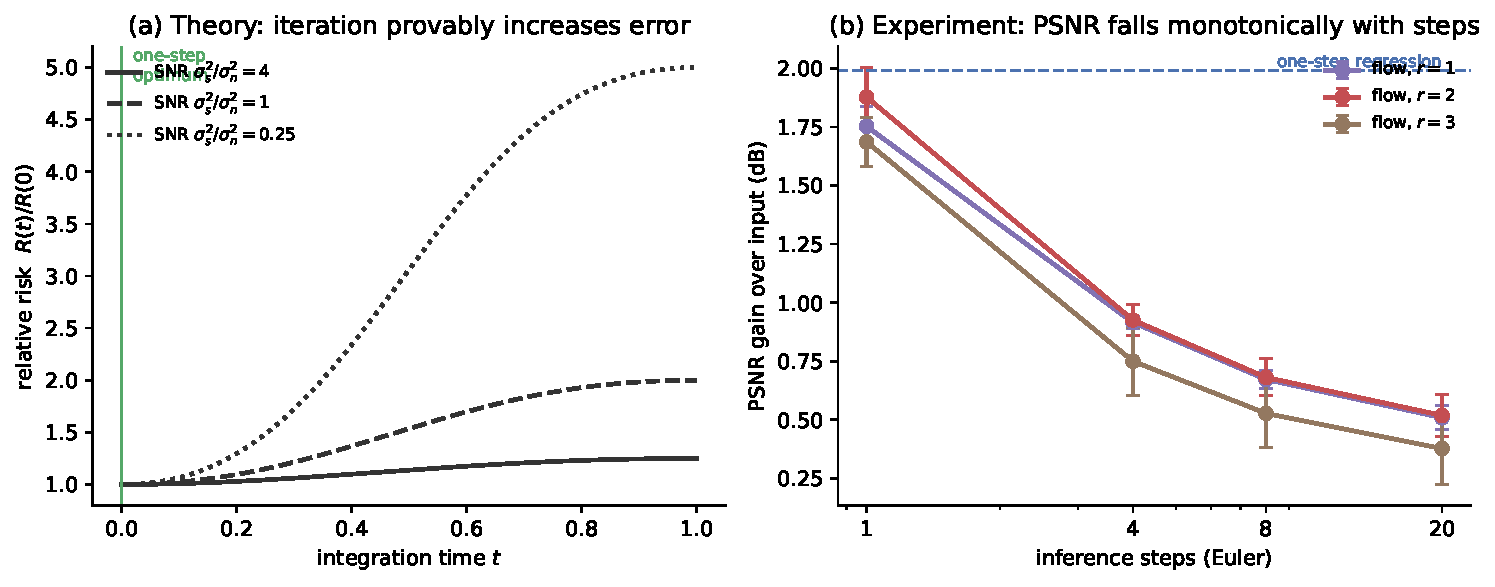
\includegraphics[width=\textwidth]{steps_departure.pdf}
  \\[4pt]
  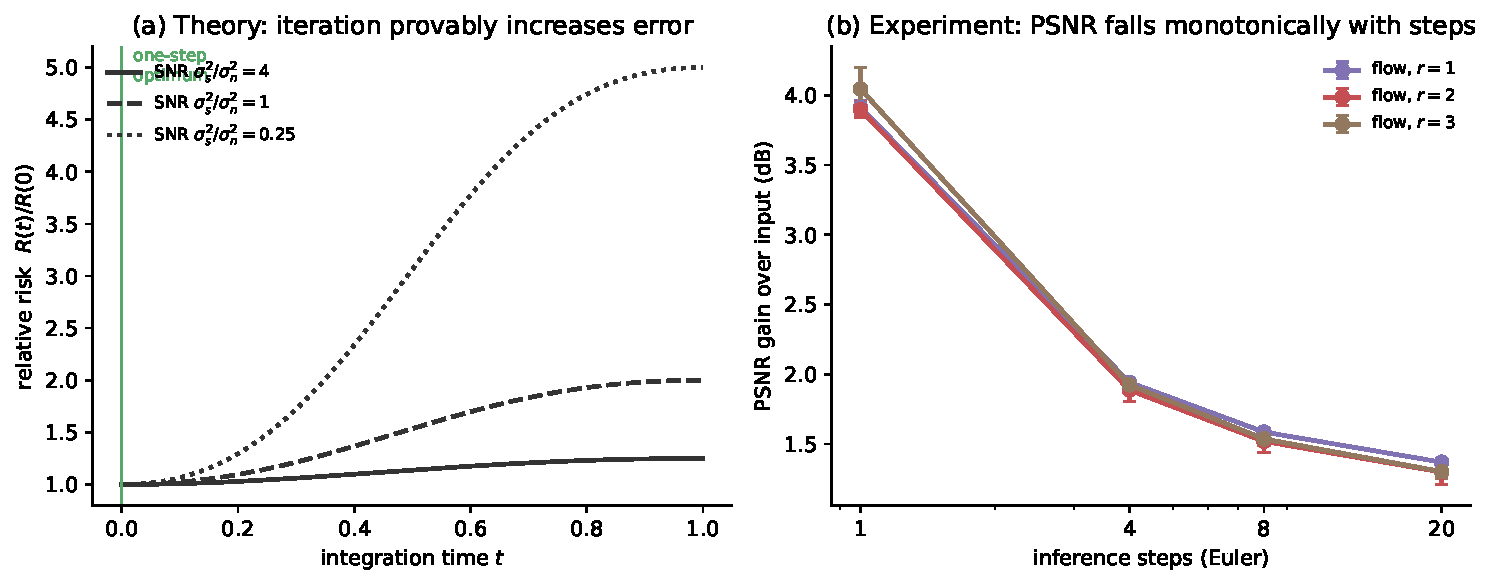
\includegraphics[width=\textwidth]{steps_departure_natural.pdf}
  \caption{\textbf{The finite-step departure, predicted and confirmed.}
           \emph{(a)} In the jointly-Gaussian model the relative denoising risk
           $R(t)/R(0)$ of the flow's readout rises monotonically with integration
           time $t$ from the one-step optimum ($t{=}0$) --- iteration
           \emph{provably} increases error (Eq.~\eqref{eq:kappa}).  \emph{(b)}
           Empirically, PSNR gain falls monotonically with the Euler step count at
           every decorrelation radius $r$ (\texttt{sweep\_hallucination.yml}, $3$
           seeds); the one-step values sit at the matched-pairing one-step
           regression baseline (dashed), which one-step flow ties.  \emph{(c)} The
           same monotone erosion on natural images (BSDS500, i.i.d.\ Gaussian
           noise; \texttt{sweep\_natural\_hallucination.yml}, $3$ seeds), with the
           natural one-step regression reference (dashed) --- the departure is not
           an artefact of CT or of correlated noise.}
  \label{fig:steps}
\end{figure*}

\subsection{Per-sweep result tables}
\label{sec:sweep-tables}
The architecture\,$\times$\,supervision benchmark (\texttt{sweep.yml}) is the
main results table, Table~\ref{tab:results} in Section~\ref{sec:results}; here we
report the flow-specific and per-image grids that drive the method.
Table~\ref{tab:ssflow-steps} is the inference-steps ablation above
(\texttt{sweep\_hallucination.yml}); Table~\ref{tab:flow-vs-reg}
(\texttt{sweep\_flow\_vs\_reg.yml}) is its regression control, holding the
similarity pairing fixed and swapping the flow estimator for a direct Noise2Sim
regressor to isolate whether the flow or the pairing is what matters.  The
per-image grid (\texttt{sweep\_periimage.yml}) is in Appendix~\ref{app:supp-tables},
Table~\ref{tab:sweep-periimage}.

\begin{table*}[t]
  \centering
  \small
  \caption{\textbf{SSFlow inference-steps ablation} (\texttt{sweep\_hallucination.yml}):
           one-step posterior mean vs.\ multi-step Euler refinement across the
           decorrelation radius $r$, on TCIA LDCT (abdomen; $3$ seeds, $50$
           epochs).  PSNR gives the absolute value with the gain over the
           $30.25$\,dB input floor.  \emph{PSNR degrades monotonically with the
           step count} at every $r$---the $20$-step gain is roughly a third of the
           one-step gain---exactly as the finite-step departure of
           Eq.~\eqref{eq:kappa} predicts, while the fabrication $d'$ holds at the
           input floor ($\approx$$0.028$) at \emph{every} step count: iteration
           erodes fidelity without inventing structure.  \textbf{Bold}: best cell
           (one-step, $r{=}2$).  $\uparrow$/$\downarrow$: higher/lower is better.}
  \label{tab:ssflow-steps}
  \begin{tabular}{ccrccccc}
    \toprule
    \textbf{Steps} & \textbf{Radius $r$} &
    PSNR\,$\uparrow$ (\,$\Delta$) & SSIM\,$\uparrow$ & RMSE\,$\downarrow$ &
    GMSD\,$\downarrow$ & RSR\,$\downarrow$ & fab.\ $d'$\,$\downarrow$ \\
    \midrule
    \multicolumn{8}{l}{\emph{Reference}} \\
    \quad LDCT input & --- & 30.25 & 0.876 & 0.0320 & 0.174 & 0.0115 & 0.028 \\
    \midrule
    \multicolumn{8}{l}{\emph{One-step posterior mean}} \\
    $1$ & $1$ & 32.00 \,(+1.75) & 0.899 & 0.0261 & 0.215 & 0.0077 & 0.030 \\
    $1$ & $2$ & \textbf{32.12 \,(+1.88)} & \textbf{0.902} & \textbf{0.0256} & 0.213 & \textbf{0.0073} & 0.029 \\
    $1$ & $3$ & 31.93 \,(+1.69) & 0.896 & 0.0261 & 0.240 & 0.0076 & 0.028 \\
    \midrule
    \multicolumn{8}{l}{\emph{Four-step Euler}} \\
    $4$ & $1$ & 31.17 \,(+0.92) & 0.889 & 0.0288 & 0.206 & 0.0095 & 0.030 \\
    $4$ & $2$ & 31.18 \,(+0.93) & 0.890 & 0.0287 & 0.204 & 0.0093 & 0.028 \\
    $4$ & $3$ & 31.00 \,(+0.75) & 0.887 & 0.0292 & 0.229 & 0.0096 & 0.028 \\
    \midrule
    \multicolumn{8}{l}{\emph{Eight-step / Twenty-step Euler}} \\
    $8$ & $2$ & 30.93 \,(+0.68) & 0.887 & 0.0295 & 0.205 & 0.0099 & 0.028 \\
    $20$ & $2$ & 30.77 \,(+0.52) & 0.885 & 0.0301 & 0.205 & 0.0103 & 0.028 \\
    \bottomrule
  \end{tabular}
\end{table*}

\begin{table*}[t]
  \centering
  \small
  \caption{\textbf{Flow-vs-regression control} (\texttt{sweep\_flow\_vs\_reg.yml}
           $+$ \texttt{sweep\_hallucination.yml}): does the one-step theorem
           (Section~\ref{sec:rf-n2n}) hold empirically?  We fix the similarity
           pairing and vary only the estimator.  The \emph{regression} arm is a
           direct Noise2Sim regressor (RED-CNN, $1.85\mathrm{M}$ params,
           capacity-comparable to SSFlow's $2.11\mathrm{M}$ velocity net); the
           \emph{flow} arm is one-step SSFlow.  Both sweep $r\in\{1,2,3\}$ over $3$
           seeds ($9$ runs each) on the identical pairs, so the arms overlay
           cell-for-cell; PSNR gain is over each split's own input floor.  \emph{The
           theorem holds:} at matched $r$ the one-step flow and the regressor agree
           to within $\le0.2$\,dB (e.g.\ $r{=}2$: $+1.88$ vs.\ $+1.99$), both
           tracing the same inverted-U that peaks at $r{=}2$---so the decorrelated
           pairing, not the estimator, is what helps.  A small residual favours
           regression (consistent with the finite-capacity caveat), so the
           decorrelated-pairing \emph{one-step regressor} at $r{=}2$
           ($+1.99$\,dB) is the best label-free result and the estimator of
           choice; the large cost is \emph{iteration}, not the objective---multi-step
           flow falls to $+0.5$\,dB (Table~\ref{tab:ssflow-steps}).  Fabrication
           $d'$ confirms neither estimator invents structure ($\approx$ input
           floor).  \textbf{Bold}: best cell.  $\uparrow$/$\downarrow$: higher/lower
           is better.}
  \label{tab:flow-vs-reg}
  \begin{tabular}{lcrccccc}
    \toprule
    \textbf{Estimator} & \textbf{Radius $r$} &
    PSNR\,$\uparrow$ (\,$\Delta$) & SSIM\,$\uparrow$ & RMSE\,$\downarrow$ &
    GMSD\,$\downarrow$ & RSR\,$\downarrow$ & fab.\ $d'$\,$\downarrow$ \\
    \midrule
    \multicolumn{8}{l}{\emph{Reference}} \\
    \quad LDCT input & --- & 30.25 & 0.876 & 0.0320 & 0.174 & 0.0115 & 0.028 \\
    \midrule
    \multicolumn{8}{l}{\emph{Regression (Noise2Sim, RED-CNN) --- same pairs, direct MMSE}} \\
    Regression & $1$ & 32.02 \,($+1.77{\pm}0.14$) & $0.900{\pm}0.015$ & $0.0260$ & $0.163$ & $0.0076$ & $0.029$ \\
    Regression & $2$ & \textbf{32.24 \,($+1.99{\pm}0.09$)} & $0.904{\pm}0.015$ & $0.0253$ & $0.160$ & $0.0071$ & $0.030$ \\
    Regression & $3$ & 32.12 \,($+1.87{\pm}0.11$) & $0.904{\pm}0.014$ & $0.0256$ & $0.162$ & $0.0072$ & $0.029$ \\
    \midrule
    \multicolumn{8}{l}{\emph{Flow (SSFlow, one-step) --- same pairs, rectified-flow objective}} \\
    Flow & $1$ & 32.00 \,($+1.75{\pm}0.08$) & $0.899{\pm}0.013$ & $0.0261$ & $0.215$ & $0.0077$ & $0.030$ \\
    Flow & $2$ & 32.12 \,($+1.88{\pm}0.13$) & $0.902{\pm}0.016$ & $0.0256$ & $0.213$ & $0.0073$ & $0.029$ \\
    Flow & $3$ & 31.93 \,($+1.69{\pm}0.10$) & $0.896{\pm}0.011$ & $0.0261$ & $0.240$ & $0.0076$ & $0.028$ \\
    \bottomrule
  \end{tabular}
\end{table*}


% -----------------------------------------------------------------------
\section{Discussion}

\paragraph{Architecture vs.\ objective.}
Under supervision the CNN backbones finish within $0.3$\,dB of one another
despite a $3\times$ parameter range, so the training objective dominates the
backbone at this budget.  The main benchmark sweep now completes both the
architecture and the objective comparison across three seeds
(Table~\ref{tab:results}).  Two backbones underperform the CNNs even
with paired targets: CTformer gains only $+1.77$\,dB and CFM $+2.84$\,dB under
supervision, versus $\sim{+}4$\,dB for RED-CNN/U-Net/DnCNN.  Because our CFM
shares the U-Net's velocity-net body, the U-Net (MSE) vs.\ CFM (flow-matching)
contrast now isolates the objective at matched capacity: the flow-matching
objective is a $\sim$1\,dB-worse route to the supervised optimum than direct MSE
regression---a supervised-regime echo of the label-free flow-vs-regression gap
that Section~\ref{sec:method} probes directly
(Table~\ref{tab:flow-vs-reg}).

\paragraph{Metric selection.}
PSNR and SSIM penalise any pixel-level deviation, even perceptually
plausible detail, systematically disadvantaging generative models; recent
reassessments show both metrics misrank restoration algorithms on medical
images~\cite{breger2025reassess} and fail to track radiologist
perception~\cite{lee2025ldctiqa}.  GMSD correlates better with perceptual
judgements~\cite{xue2014gradient}, and RSR is directly interpretable by
radiologists as a frequency-domain characterisation of residual noise.  The
stronger standard---task-based detectability via a model
observer~\cite{li2021detection,kc2024lgcho}, together with explicit
hallucination quantification~\cite{bhadra2021halluc,tivnan2024halluc}---is
reported in Section~\ref{sec:detect}: on these benchmark models the CHO
confirms that the PSNR/SSIM gains overstate task performance, with
low-contrast detectability eroded rather than improved.  We recommend future
CT-denoising work report task-based $d'$ alongside the five metrics in
Table~\ref{tab:results}.

\paragraph{Limitations.}
The \emph{clinical} evaluation---the benchmark and the detectability study---is
$3$-seed and patient-level but on the abdomen window only for the $3$-seed
numbers; the supervision-regime ordering additionally reproduces on an
independent, simulated low-dose source of the same anatomy
(Table~\ref{tab:sim-ldct}) and, at single seed, on a second anatomy (chest,
Table~\ref{tab:chest}), leaving a $3$-seed chest replication as the primary
remaining strengthening for the CT-specific numbers.  The \emph{theoretical}
claim is less domain-bound: the one-step-optimality and finite-step-departure
findings reproduce on natural images under i.i.d.\ Gaussian noise
(Table~\ref{tab:natural}), so they are not artefacts of CT or of correlated noise.
The per-image methods (ZS-N2N, Filter2Noise) are reported single-split
(Appendix~\ref{app:supp-tables}); their $3$-seed and detectability numbers are
omitted because each CHO realisation would retrain their per-image network
thousands of times.  The finite-step departure result
(Section~\ref{sec:ss-pairs}) is proved exactly only in the jointly-Gaussian model;
a bound for the general finite-capacity, finite-step case is left open, though the
CT and natural-image experiments both exhibit the predicted monotone erosion
outside that model's assumptions.  Detectability is
reported for the deterministic denoisers and, through the fabrication-vs-steps
pass, for the generative SSFlow; a broader hallucination analysis of generative
CT denoisers is a natural extension.

% -----------------------------------------------------------------------
\section{Conclusion}

We presented CTDenoiser, a benchmark that trains and evaluates five LDCT
denoising architectures under a shared, reproducible harness with a
corrected full-slice evaluation and two CT-appropriate metrics (GMSD,
RSR).  Once the evaluation is corrected, supervised denoisers gain
$\sim$4\,dB over the noisy input, and among label-free methods only the
correlated-noise-aware Noise2Sim reliably beats it while blind-spot
Noise2Void degrades, leaving a $\sim$2\,dB gap to supervised.  Our central
methodological contribution is a proof that an \emph{unconditional} rectified
flow, trained on two noisy observations of the same signal, recovers the
Noise2Noise posterior mean in a single step without clean targets, together with
a finite-step departure result showing any multi-step integration provably
worsens it.  A matched-pairing experiment confirms both: one-step flow ties a
direct regressor while multi-step Euler integration monotonically erodes
fidelity, so the decorrelated \emph{pairing}, not the flow machinery, is the
useful idea, and a one-step regressor on those pairs is our best label-free
result ($+1.99$\,dB).  All code is released to facilitate reproducibility.

% ===== References (extra pages permitted by AAAI) =====
% Bibliography is maintained in refs.bib; the AAAI style file selects
% \bibliographystyle{aaai2026} automatically when natbib is loaded.
\bibliography{refs}

% ===== Supplementary material: after references; not counted in the 7-page limit =====
\appendix

\section{Robustness experiments}
\label{app:robustness}
The benchmark ordering is corroborated on two further axes below: an
independent \emph{simulated} low-dose source (same anatomy) and a second
\emph{anatomy} (chest). Both are summarised in the Limitations paragraph of
the main text.

\subsection{Robustness to a second LDCT source}
\label{sec:sim-ldct}
The main benchmark (Table~\ref{tab:results}) draws its low-dose arm from one real
acquisition.  To check that the supervision-regime ordering is a property of
correlated LDCT noise rather than of that single acquisition, we re-run the same
architecture\,$\times$\,supervision grid on an independent low-dose source
(\texttt{sweep\_sim\_ldct.yml}): the low-dose images are \emph{simulated} from the
same abdomen full-dose volumes with a correlated, signal-dependent noise model
(\texttt{-{}-sim-base-std=0.03}, \texttt{-{}-sim-signal-std=0.06}), giving a
harsher $28.3$\,dB input floor (vs.\ $30.25$\,dB real).  Everything else---patient
splits, patch size, optimiser, seeds, epochs---is held fixed.

The regime ordering reproduces on the second source
(Table~\ref{tab:sim-ldct}): supervised denoising gains $\sim$$4.5$--$4.9$\,dB with
the three CNNs again within $0.4$\,dB of one another; among label-free methods
Noise2Sim is the \emph{only} one that clears the noisy floor at every backbone,
while blind-spot Noise2Void is flat-to-negative ($-0.09$ to $+0.04$\,dB).  The
qualitative story is therefore source-independent.  Two magnitudes shift with the
noise model, in the direction the mechanism predicts: Noise2Sim's margin
\emph{compresses} to $+0.9$\,dB (from $+1.8$\,dB on the real source), because the
simulated field is more nearly stationary and leaves the similarity search less
correlation structure to exploit; and Noise2Void moves toward---rather than
below---the floor, as a milder correlation length lessens (without removing) its
pixel-independence violation.  The ordering is robust; the label-free margin is
source-dependent, which we report rather than average away.

\begin{table*}[t]
  \centering
  \small
  \caption{\textbf{Robustness to a second LDCT source} (\texttt{sweep\_sim\_ldct.yml}):
           the Table~\ref{tab:results} grid re-run with the low-dose arm
           \emph{simulated} from the abdomen full-dose volumes (correlated,
           signal-dependent noise; $3$ seeds, $50$ epochs, matched splits).  PSNR
           gives the absolute value with the gain over the $28.26$\,dB simulated
           input floor in parentheses.  The supervision-regime ordering matches the
           real-source benchmark---supervised $\sim$$4.5$--$4.9$\,dB, Noise2Sim the
           only label-free method above the floor, Noise2Void flat-to-negative---so
           it is not an artefact of one acquisition; the label-free margin
           compresses under the more stationary simulated noise.  \textbf{Bold}:
           best $\Delta$PSNR per supervision block.  $^{\dagger}$Two CTformer runs
           crashed near convergence (epoch $47$--$49$), leaving supervised at
           $2/3$ and Noise2Void at $1/3$ seeds (shown without s.d.); all other
           cells are $3$ seeds.  $\uparrow$/$\downarrow$: higher/lower is better.}
  \label{tab:sim-ldct}
  \begin{tabular}{llrccccc}
    \toprule
    \textbf{Model} & \textbf{Supervision} & \textbf{Params} &
    PSNR\,$\uparrow$ (\,$\Delta$) & SSIM\,$\uparrow$ & RMSE\,$\downarrow$ &
    GMSD\,$\downarrow$ & RSR\,$\downarrow$ \\
    \midrule
    Simulated LDCT input & --- (no denoising) & --- & $28.26$ & $0.597$ & $0.0388$ & $0.418$ & $0.0153$ \\
    \midrule
    RED-CNN~\cite{chen2017lowdose}   & Supervised & $1.85\mathrm{M}$ & \textbf{33.17 \,($+4.91{\pm}0.13$)} & $0.937$ & $0.0221$ & $0.169$ & $0.0050$ \\
    DnCNN~\cite{zhang2017beyond}     & Supervised & $0.56\mathrm{M}$ & 32.90 \,($+4.64{\pm}0.14$) & $0.934$ & $0.0228$ & $0.222$ & $0.0053$ \\
    U-Net                            & Supervised & $1.95\mathrm{M}$ & 32.78 \,($+4.52{\pm}0.11$) & $0.933$ & $0.0231$ & $0.222$ & $0.0055$ \\
    CTformer$^{\dagger}$~\cite{wang2022ctformer} & Supervised & $0.40\mathrm{M}$ & 30.22 \,($+1.96{\pm}0.04$) & $0.860$ & $0.0309$ & $0.361$ & $0.0098$ \\
    CFM~\cite{lipman2022flow}        & Supervised & $2.11\mathrm{M}$ & 31.07 \,($+2.81{\pm}0.17$) & $0.914$ & $0.0281$ & $0.226$ & $0.0081$ \\
    \midrule
    RED-CNN~\cite{chen2017lowdose}   & Noise2Sim~\cite{niu2020noise2sim} & $1.85\mathrm{M}$ & \textbf{29.22 \,($+0.96{\pm}0.07$)} & $0.706$ & $0.0347$ & $0.409$ & $0.0123$ \\
    U-Net                            & Noise2Sim~\cite{niu2020noise2sim} & $1.95\mathrm{M}$ & 29.19 \,($+0.93{\pm}0.05$) & $0.673$ & $0.0348$ & $0.384$ & $0.0124$ \\
    DnCNN~\cite{zhang2017beyond}     & Noise2Sim~\cite{niu2020noise2sim} & $0.56\mathrm{M}$ & 29.11 \,($+0.85{\pm}0.05$) & $0.667$ & $0.0351$ & $0.395$ & $0.0126$ \\
    CTformer~\cite{wang2022ctformer} & Noise2Sim~\cite{niu2020noise2sim} & $0.40\mathrm{M}$ & 28.81 \,($+0.55{\pm}0.09$) & $0.810$ & $0.0364$ & $0.346$ & $0.0135$ \\
    \midrule
    RED-CNN~\cite{chen2017lowdose}   & Noise2Void~\cite{krull2019noise2void} & $1.85\mathrm{M}$ & \textbf{28.30 \,($+0.04{\pm}0.09$)} & $0.643$ & $0.0386$ & $0.398$ & $0.0152$ \\
    DnCNN~\cite{zhang2017beyond}     & Noise2Void~\cite{krull2019noise2void} & $0.56\mathrm{M}$ & 28.24 \,($-0.02{\pm}0.04$) & $0.627$ & $0.0389$ & $0.390$ & $0.0154$ \\
    U-Net                            & Noise2Void~\cite{krull2019noise2void} & $1.95\mathrm{M}$ & 28.17 \,($-0.09{\pm}0.08$) & $0.646$ & $0.0391$ & $0.381$ & $0.0157$ \\
    CTformer$^{\dagger}$~\cite{wang2022ctformer} & Noise2Void~\cite{krull2019noise2void} & $0.40\mathrm{M}$ & 28.04 \,($-0.20$) & $0.723$ & $0.0397$ & $0.342$ & $0.0163$ \\
    \bottomrule
  \end{tabular}
\end{table*}

\subsection{Robustness to a second anatomy}
\label{sec:chest}
The simulated-source check varies the noise model but holds the anatomy fixed.
To vary the \emph{anatomy}, we re-run the benchmark grid on a chest LDCT cache
(real low/full-dose pairs, $10$ patients, $8$ train / $2$ val; a single seed --- a
fast ordering check, not a significance table).  The supervision-regime ordering
reproduces on the CNNs (Table~\ref{tab:chest}): supervised leads (RED-CNN
$+3.29$\,dB over the $39.68$\,dB chest floor), Noise2Sim is again the \emph{only}
label-free method clearly above the floor (RED-CNN $+1.52$), and Noise2Void is
flat-to-negative.  The task-based erosion reproduces too, and is if anything
sharper: supervised RED-CNN preserves only $0.46$ of the input's low-contrast
detectability despite the $+3.3$\,dB.  Two cohort-specific caveats: gains are
compressed and noisier than abdomen because the chest floor is high ($39.68$ vs.\
$30.25$\,dB) and only one seed is run; and the data-hungry CTformer diverged on
the $8$-patient training set (all modes below the floor), so it is omitted here.
A $3$-seed chest replication is the main remaining strengthening.

\begin{table*}[t]
  \centering
  \small
  \caption{\textbf{Robustness to a second anatomy} (\texttt{sweep\_chest.yml}):
           the Table~\ref{tab:results} grid on a chest LDCT cache (real
           low/full-dose pairs, $10$ patients, \emph{single seed}) instead of
           abdomen.  PSNR gives the absolute value with the gain over the
           $39.68$\,dB chest input floor in parentheses.  The CNN supervision
           ordering reproduces---supervised leads, Noise2Sim the only label-free
           method above the floor, Noise2Void flat-to-negative---though gains are
           compressed by the high chest floor and noisier at single seed.  CTformer
           diverged on the $8$-patient chest cohort (all modes below the floor) and
           is omitted; CFM requires paired targets and so appears only under
           supervision.  \textbf{Bold}: best $\Delta$PSNR per supervision block.
           $\uparrow$/$\downarrow$: higher/lower is better.}
  \label{tab:chest}
  \begin{tabular}{llrccccc}
    \toprule
    \textbf{Model} & \textbf{Supervision} & \textbf{Params} &
    PSNR\,$\uparrow$ (\,$\Delta$) & SSIM\,$\uparrow$ & RMSE\,$\downarrow$ &
    GMSD\,$\downarrow$ & RSR\,$\downarrow$ \\
    \midrule
    Chest LDCT input & --- (no denoising) & --- & $39.68$ & $0.932$ & $0.0110$ & $0.235$ & $0.0004$ \\
    \midrule
    RED-CNN~\cite{chen2017lowdose}   & Supervised & $1.85\mathrm{M}$ & \textbf{42.97 \,($+3.29$)} & $0.970$ & $0.0075$ & $0.209$ & $0.0002$ \\
    CFM~\cite{lipman2022flow}        & Supervised & $2.11\mathrm{M}$ & 41.97 \,($+2.29$) & $0.965$ & $0.0084$ & $0.206$ & $0.0002$ \\
    DnCNN~\cite{zhang2017beyond}     & Supervised & $0.56\mathrm{M}$ & 41.70 \,($+2.02$) & $0.959$ & $0.0088$ & $0.216$ & $0.0002$ \\
    U-Net                            & Supervised & $1.95\mathrm{M}$ & 41.01 \,($+1.33$) & $0.965$ & $0.0092$ & $0.207$ & $0.0002$ \\
    \midrule
    RED-CNN~\cite{chen2017lowdose}   & Noise2Sim~\cite{niu2020noise2sim} & $1.85\mathrm{M}$ & \textbf{41.20 \,($+1.52$)} & $0.954$ & $0.0092$ & $0.219$ & $0.0003$ \\
    U-Net                            & Noise2Sim~\cite{niu2020noise2sim} & $1.95\mathrm{M}$ & 40.09 \,($+0.41$) & $0.959$ & $0.0102$ & $0.212$ & $0.0003$ \\
    DnCNN~\cite{zhang2017beyond}     & Noise2Sim~\cite{niu2020noise2sim} & $0.56\mathrm{M}$ & 39.85 \,($+0.17$) & $0.935$ & $0.0107$ & $0.232$ & $0.0004$ \\
    \midrule
    U-Net                            & Noise2Void~\cite{krull2019noise2void} & $1.95\mathrm{M}$ & \textbf{39.62 \,($-0.05$)} & $0.959$ & $0.0107$ & $0.212$ & $0.0003$ \\
    RED-CNN~\cite{chen2017lowdose}   & Noise2Void~\cite{krull2019noise2void} & $1.85\mathrm{M}$ & 39.38 \,($-0.30$) & $0.949$ & $0.0111$ & $0.223$ & $0.0003$ \\
    DnCNN~\cite{zhang2017beyond}     & Noise2Void~\cite{krull2019noise2void} & $0.56\mathrm{M}$ & 38.03 \,($-1.65$) & $0.929$ & $0.0129$ & $0.240$ & $0.0005$ \\
    \bottomrule
  \end{tabular}
\end{table*}

\section{Supplementary Tables}
\label{app:supp-tables}

Two supporting tables referenced from the main text: the reduced-budget
cross-validation that confirms the per-fold stability of the benchmark ordering
(Table~\ref{tab:cv}, Section~\ref{sec:results}) and the per-image, test-time
methods (Table~\ref{tab:sweep-periimage}).

\begin{table*}[t]
  \centering
  \small
  \caption{Three-fold patient-level cross-validation on TCIA LDCT (abdomen;
           15 epochs).  $\Delta$PSNR and SSIM are the mean ($\pm$ s.d.) across
           the three folds; the PSNR gain is measured against each fold's own
           LDCT-input floor ($31.44/30.04/29.27$\,dB for folds $1/2/3$).  PSNR,
           RMSE, and RSR are fold means.  Only DnCNN and RED-CNN completed
           all three folds and are shown; U-Net had incomplete fold coverage at
           export.  Filter2Noise and ZS-N2N are per-image and model-agnostic
           (single row each).  \textbf{Bold}: best per column.
           \underline{Underline}: best \emph{label-free} PSNR gain.}
  \label{tab:cv}
  \begin{tabular}{llccccc}
    \toprule
    \textbf{Model} & \textbf{Supervision} &
    $\Delta$PSNR\,$\uparrow$ (dB) & PSNR\,$\uparrow$ & SSIM\,$\uparrow$ &
    RMSE\,$\downarrow$ & RSR\,$\downarrow$ \\
    \midrule
    RED-CNN~\cite{chen2017lowdose} & Supervised & \textbf{+4.19 $\pm$ 0.22} & \textbf{34.43} & \textbf{0.927 $\pm$ 0.013} & \textbf{0.0195} & \textbf{0.0042} \\
    DnCNN~\cite{zhang2017beyond}   & Supervised & +4.04 $\pm$ 0.22 & 34.29 & 0.924 $\pm$ 0.015 & 0.0199 & 0.0044 \\
    \midrule
    RED-CNN~\cite{chen2017lowdose} & Noise2Sim~\cite{niu2020noise2sim} & \underline{+1.74 $\pm$ 0.09} & 31.99 & 0.900 $\pm$ 0.015 & 0.0261 & 0.0077 \\
    DnCNN~\cite{zhang2017beyond}   & Noise2Sim~\cite{niu2020noise2sim} & +1.42 $\pm$ 0.28 & 31.66 & 0.895 $\pm$ 0.015 & 0.0271 & 0.0082 \\
    \midrule
    RED-CNN~\cite{chen2017lowdose} & Noise2Void~\cite{krull2019noise2void} & +0.32 $\pm$ 0.10 & 30.57 & 0.883 $\pm$ 0.019 & 0.0306 & 0.0105 \\
    DnCNN~\cite{zhang2017beyond}   & Noise2Void~\cite{krull2019noise2void} & $-0.02$ $\pm$ 0.06 & 30.23 & 0.875 $\pm$ 0.018 & 0.0320 & 0.0114 \\
    \midrule
    Filter2Noise~\cite{sun2025filter2noise} & Zero-shot & +0.26 $\pm$ 0.11 & 30.51 & 0.881 $\pm$ 0.016 & 0.0309 & 0.0105 \\
    ZS-N2N~\cite{mansour2023zsn2n}          & Zero-shot & $-0.09$ $\pm$ 0.20 & 30.16 & 0.879 $\pm$ 0.015 & 0.0319 & 0.0112 \\
    \bottomrule
  \end{tabular}
\end{table*}

\begin{table*}[t]
  \centering
  \small
  \caption{\textbf{Per-image sweep} (\texttt{sweep\_periimage.yml}): test-time,
           data-free methods, model-agnostic.  Values shown are single-split
           seed-0 (floor $31.44$\,dB; $\Delta$ over that floor); the $3$-seed
           means ($2$ modes $\times$ $3$ seeds) are pending and will match the
           benchmark's $30.25$\,dB floor.  Both methods sit essentially at the
           noisy floor---consistent with the label-free ordering in
           Table~\ref{tab:results}.  $\uparrow$/$\downarrow$: higher/lower is
           better.}
  \label{tab:sweep-periimage}
  \begin{tabular}{llrccccc}
    \toprule
    \textbf{Method} & \textbf{Type} & \textbf{Params} &
    PSNR\,$\uparrow$ (\,$\Delta$) & SSIM\,$\uparrow$ & RMSE\,$\downarrow$ &
    GMSD\,$\downarrow$ & RSR\,$\downarrow$ \\
    \midrule
    Filter2Noise~\cite{sun2025filter2noise} & Zero-shot & --- & 31.58 \,(+0.14) & 0.896 & 0.0269 & 0.176 & 0.0076 \\
    ZS-N2N~\cite{mansour2023zsn2n}          & Zero-shot & $21.3\mathrm{K}$ & 31.17 \,($-0.27$) & 0.892 & 0.0281 & 0.182 & 0.0083 \\
    \bottomrule
  \end{tabular}
\end{table*}

\section{Reproducibility Checklist}
\label{app:repro}
This paper makes both theoretical and experimental contributions.
\emph{Theory:} all claims (the one-step Noise2Noise/MMSE identity and the
finite-step departure, Section~4) state their assumptions and include complete
proofs in the jointly-Gaussian model.
\emph{Data:} all experiments use public datasets---the TCIA Low-Dose CT and
Projection benchmark and BSDS500 natural images---with the patient-level splits,
HU windows, and preprocessing given in Section~3.1.
\emph{Code:} the full training loop, model definitions, evaluation harness
(overlapped tiling, CHO detectability, NPS), and every sweep configuration will
be released openly (repository link withheld for anonymous review).
\emph{Compute and settings:} architectures, parameter counts, optimiser, epochs,
seeds ($3$ unless noted), and patch/batch sizes are reported in Section~3 and the
table captions; results are mean\,$\pm$\,s.d.\ over $3$ seeds except the
single-seed chest robustness check, which is labelled as such.

\end{document}
